\documentclass[landscape,12pt,openany]{book}

\usepackage{multicol}
\usepackage{graphicx}
\graphicspath{{./images/}}
\usepackage[margin=.5in, paperwidth=9in, paperheight=7in]{geometry}
\usepackage{titlesec}
\usepackage{xfrac}

\titlespacing*{\chapter}{0pt}{-50pt}{20pt}
\titleformat{\chapter}[display]{\normalfont\huge\bfseries}{\chaptertitlename\
\thechapter}{20pt}{\Huge}
\setlength{\columnseprule}{0.4pt}
\pagestyle{plain}

\begin{document}

\title{Cookbook}
\author{Chase Seibert}
\maketitle

\columnsep=2em
\setlength{\columnseprule}{0pt}.

\cleardoublepage
\tableofcontents
\chapter{Salads}

\section{Caesar Salad}
\begin{multicols*}{3}

Place serving bowls and large mixing bowl in the freezer.

\begin{tabular}{r@{ }l}
    \sfrac{1}{2} & loaf rustic bread \\
    \sfrac{1}{2} & stick butter \\
                 & garlic powder (granules) \\
\end{tabular}

Cut bread into ½ inch cubes, sauté  with butter until saturated. Spread on a baking sheet and sprinkle liberally with garlic powder.

Bake at 350 for 10 minutes, and then continue to bake watching closely until golden brown.
Place croûtons in an open container and put in the freezer for 10 minutes.

\begin{tabular}{r@{ }l}
    block parmesan reggiano \\
\end{tabular}

Grate 1 cup coarse, and ½ cup fine.

\begin{tabular}{r@{ }l}
    2 & heads romaine hearts \\
\end{tabular}

Cut into ¾ inch rounds, separate and then chop roughly.

\begin{tabular}{r@{ }l}
    dressing \\
    fresh pepper \\
\end{tabular}

When you're ready to serve, remove large mixing bowl from freezer. Combine lettuce, cheese, pepper and two large spoon fulls of dressing.
Add croûtons, and mix again briefly. Turn out into serving bowls from the freezer.
This must be served immediately. In just a few minutes, the salad will start turning greasy and limp.
Caesar Dressing

\begin{tabular}{r@{ }l}
               1 & large egg \\
               3 & tablespoons lemon juice \\
               1 & teaspoon Worcestershire \\
   1\sfrac{1}{2} & teaspoon anchovy paste \\
               1 &  clove garlic \\
\end{tabular}

Blanch egg in shell for 45 seconds in boiling water. Remove and crack into a small bowl. Whisk with other ingredients.

\begin{tabular}{r@{ }l}
    \sfrac{1}{3} & cup olive oil (extra-virgin) \\
\end{tabular}

Slowly whisk oil into the dressing. Season to taste with salt and pepper.

\end{multicols*}
\clearpage

\newgeometry{margin=0in}
\begin{figure}[p]
    \centering
    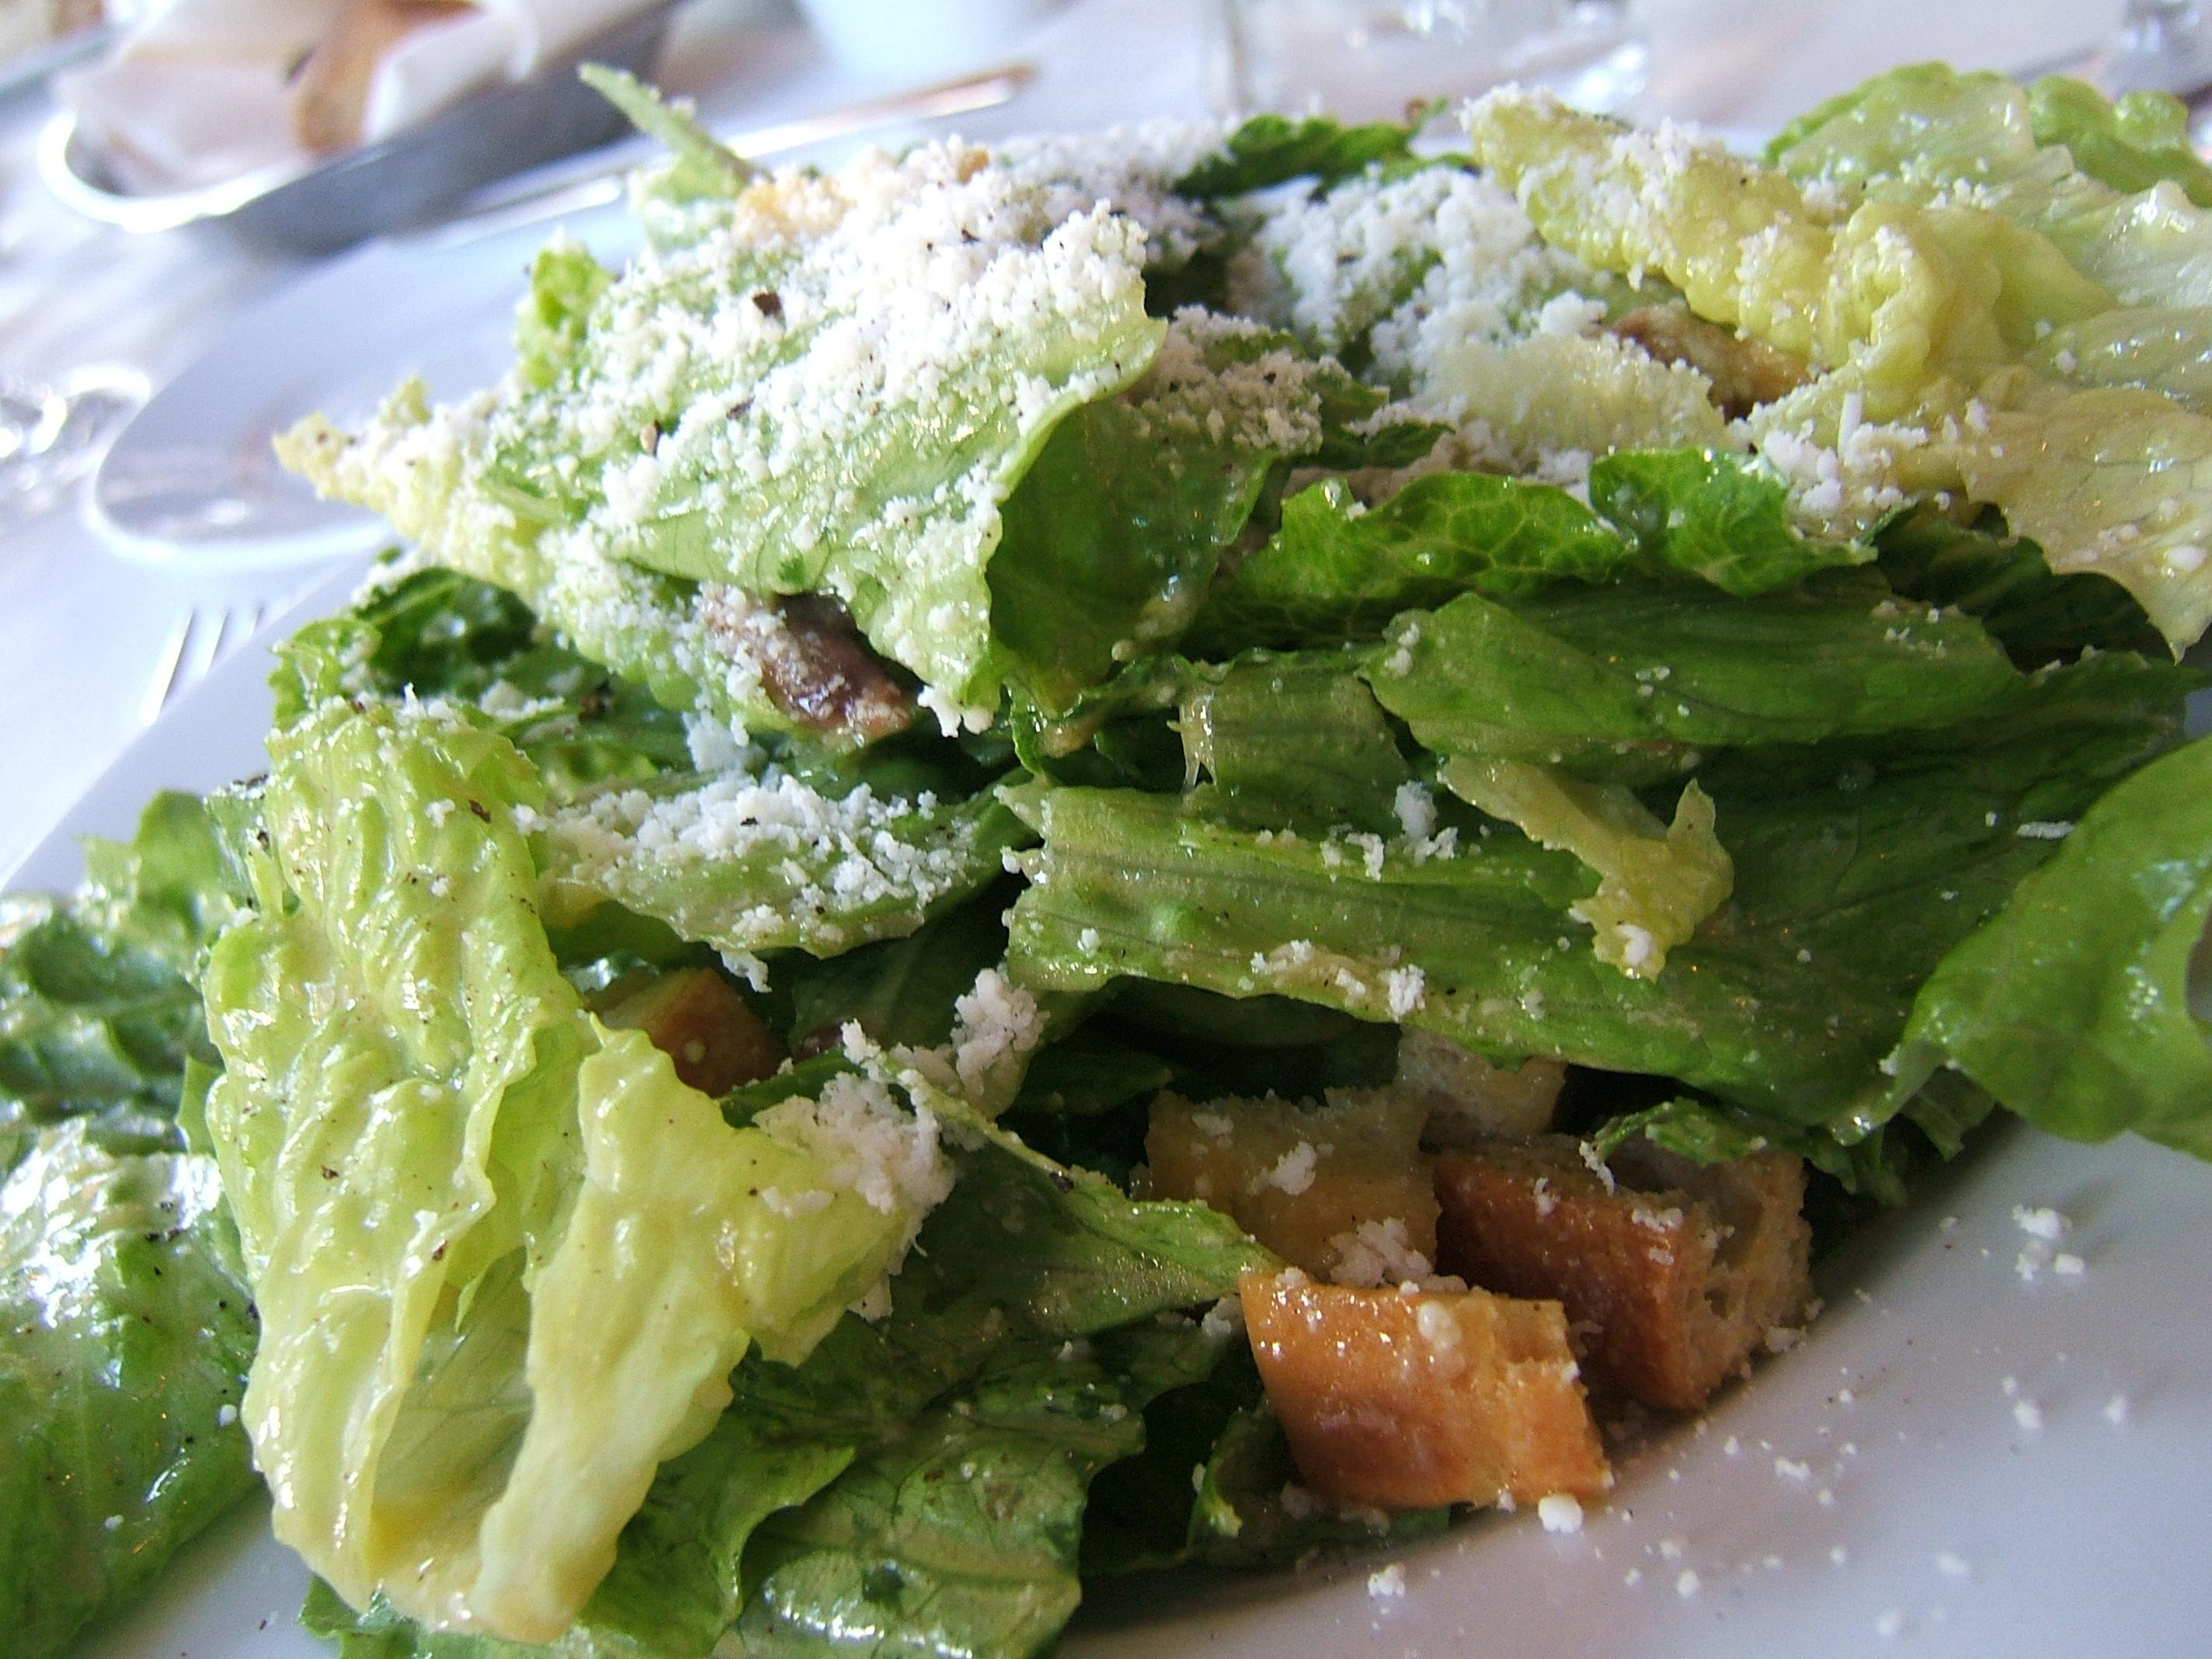
\includegraphics[width=\paperwidth,height=\paperheight]{caesar2.jpg}
    \caption{Caesar Salad}
\end{figure}
\restoregeometry

\clearpage


\section{Anne's Spinach Salad}
\begin{multicols*}{3}

\begin{quote}
    This recipe is from my Aunt Anne, who swears that she always used romaine lettuce instead of spinach.
\end{quote}

\begin{tabular}{r@{ }l}
    2 & eggs \\
\end{tabular}

Boil eggs, cool, shell and slice into rings.

\begin{tabular}{r@{ }l}
    10 & strips bacon \\
\end{tabular}

Separate strips onto aluminum foil in a baking sheet, and bake for 15 minutes at 425. Pat dry and chop into small pieces.

\begin{tabular}{r@{ }l}
    \sfrac{1}{2} & cup olive oil \\
    \sfrac{3}{4} & can anchovies in oil \\
               2 & tablespoons balsamic \\
               2 & tablespoons lemon juice \\
               1 & garlic clove \\
    \sfrac{1}{2} & teaspoon thyme \\
    \sfrac{1}{4} & teaspoon \\
                 & sugar \\
                 & oregano \\
                 & mustard powder \\
                 & onion salt \\
                 & paprika \\
\end{tabular}

Discard the oil in the can and use only the anchovies. Liquefy all  ingredients in a blender.

\begin{tabular}{r@{ }l}
    1 & package spinach \\
      & pre-sliced mushrooms \\
\end{tabular}

Combine eggs, bacon and dressing in a large mixing bowl.

\begin{quote}
The dressing can keep at least overnight.

To shell eggs easily, run under cold water, shaking pan to smash shells. The water will seep in. In 10 minutes, the shells will come off easily.

Leftover spinach can be saved, but be sure to reseal it in the original packaging, which is specially designed to breath. Spinach or lettuce saved in regular plastic will rot in a few days.

If you want to chop bacon very fine, freeze it for 10 minutes first.
\end{quote}

\end{multicols*}

\clearpage

\newgeometry{margin=0in}
\begin{figure}[p]
    \centering
    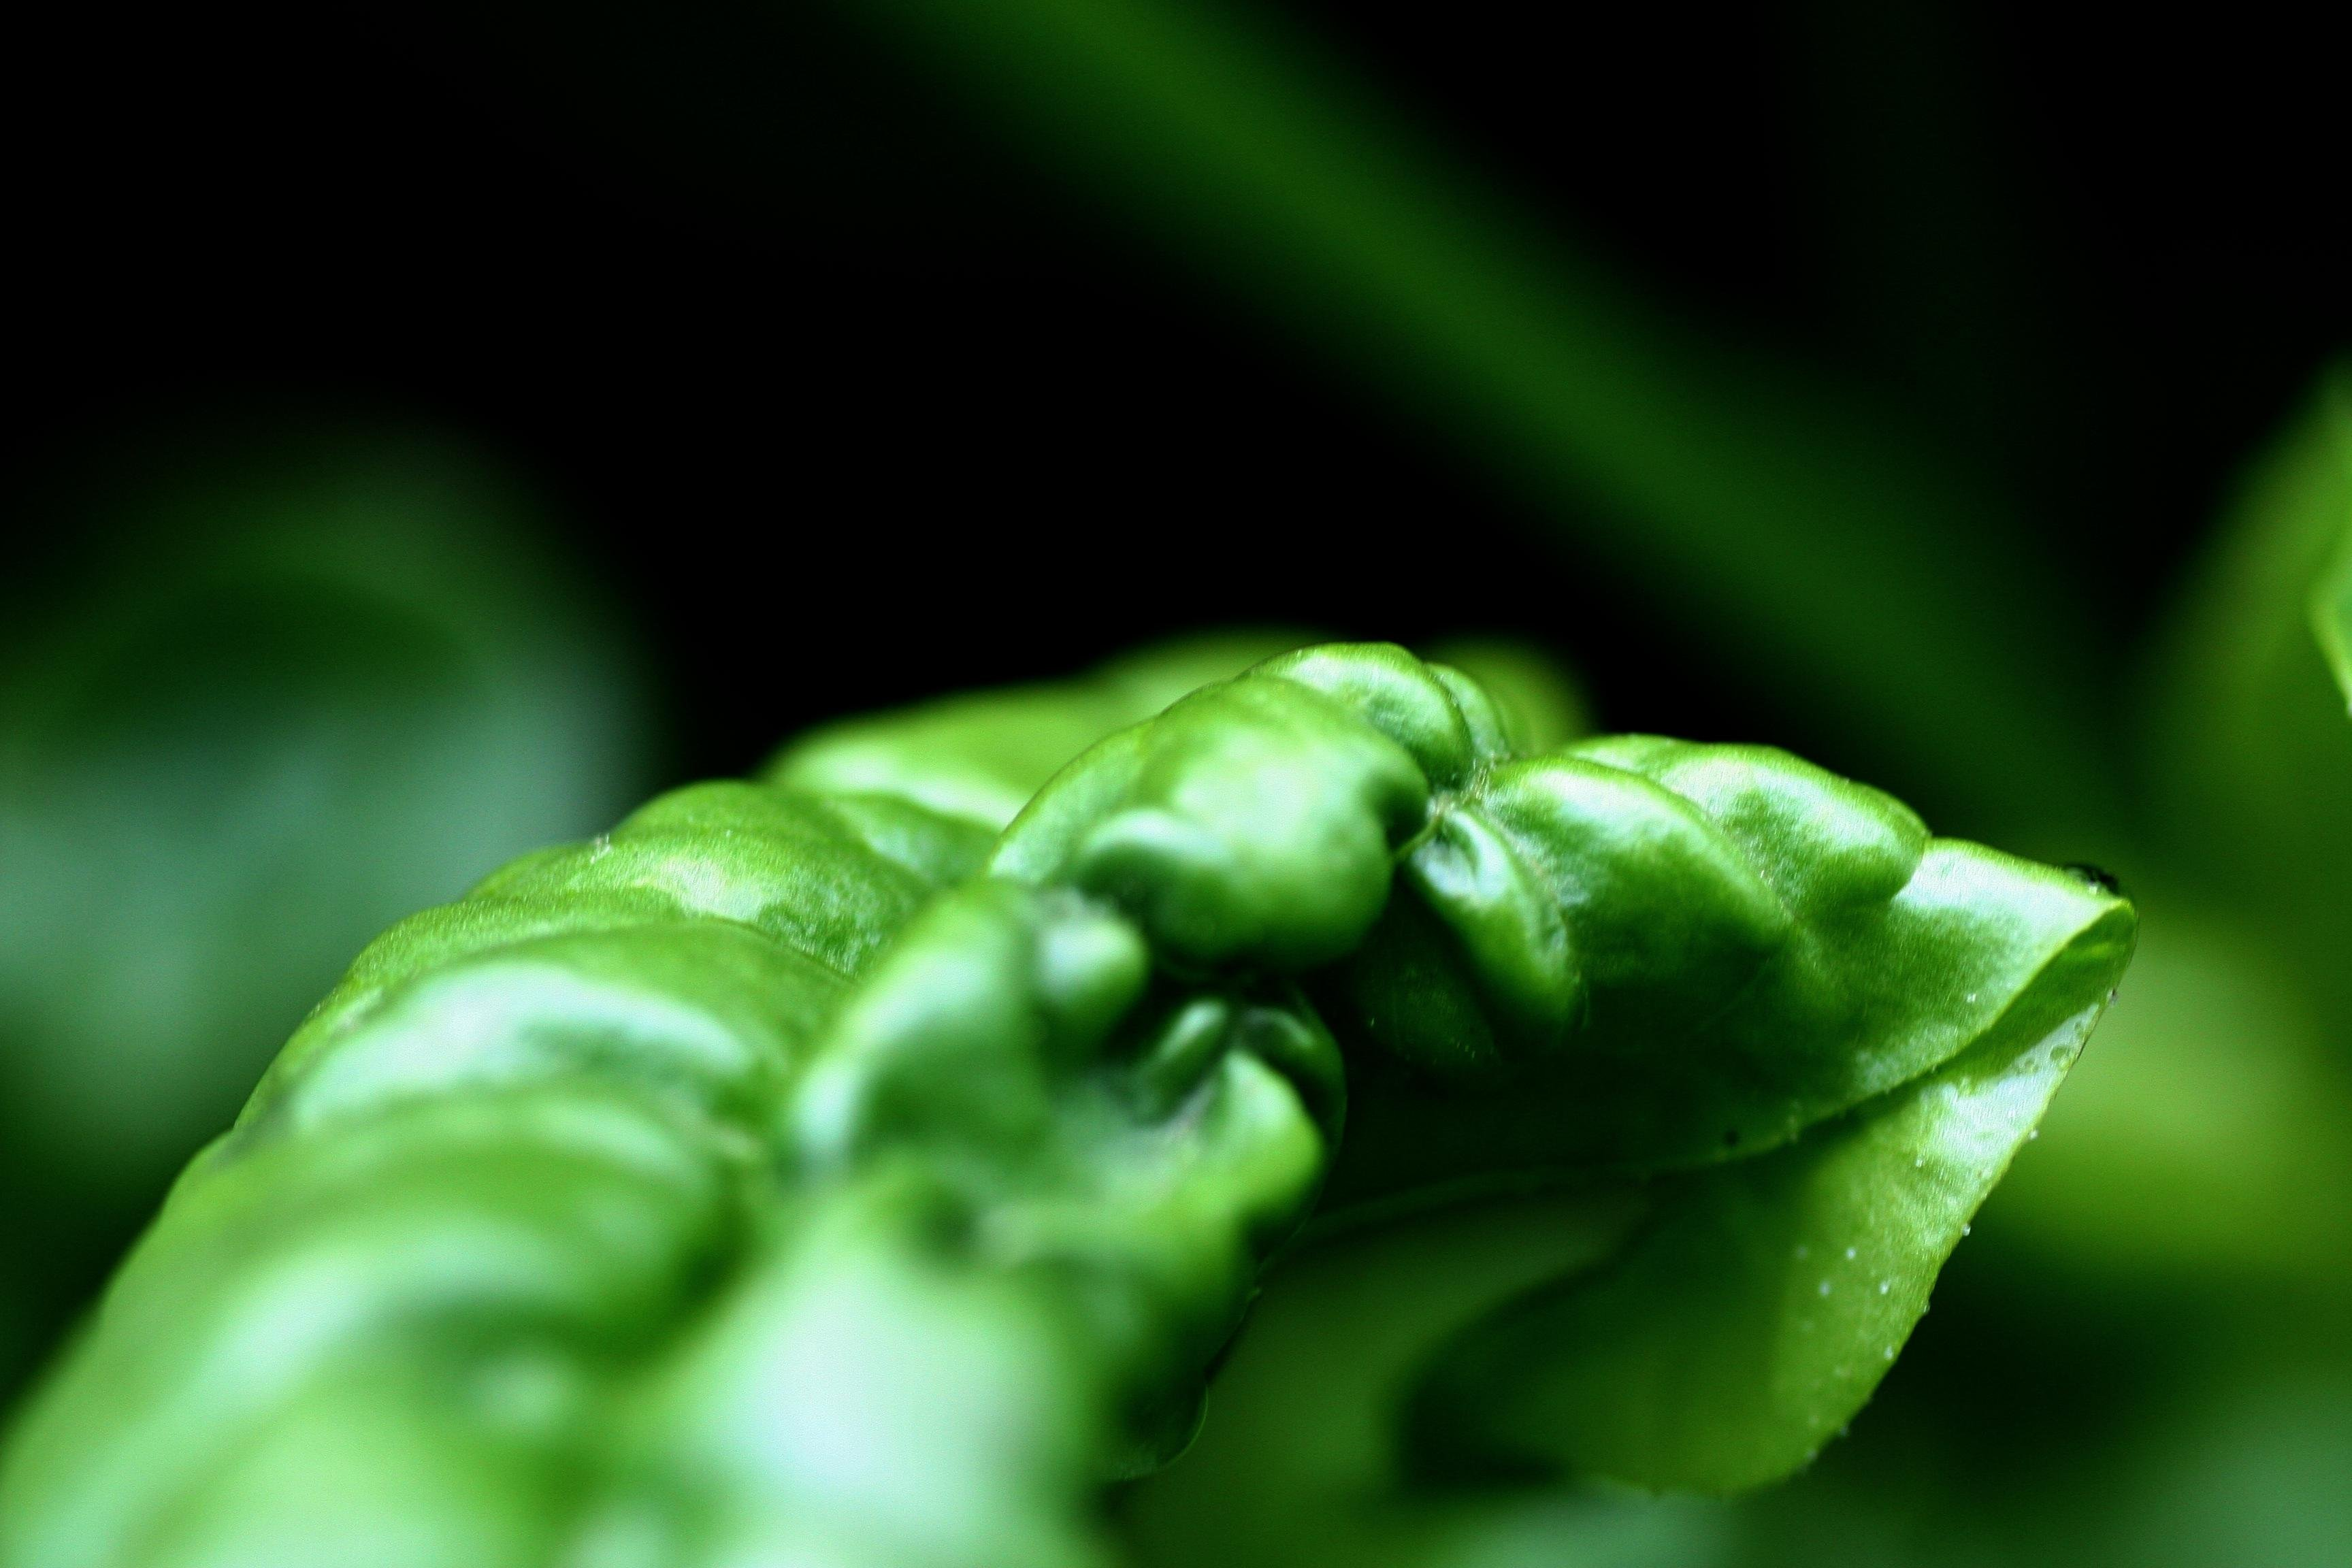
\includegraphics[width=\paperwidth,height=\paperheight]{spinach.jpg}
    \caption{Fresh Spinach}
\end{figure}
\restoregeometry

\clearpage

\listoffigures

\end{document}

- separate tex files per recipe?
- make macros (?) for images, lists, etc to reduce redundancy. DRY
    create own package (sty file)
- tips styling
- custom title pages (section 7.2)
- reduce chapter title height
- image attribution
- better fonts
